\documentclass[12pt,a4paper]{article}

\usepackage{amsmath} % у преамбулі

\usepackage[utf8]{inputenc}
\usepackage[T2A]{fontenc}
\usepackage[ukrainian]{babel}
\usepackage{graphicx} % <-- Для роботи з \includegraphics
\usepackage{geometry}
\geometry{
    left=2cm,
    right=2cm,
    top=2cm,
    bottom=2cm
}

\begin{document}

    \begin{titlepage}

        \thispagestyle{empty}
        \begin{center}
        \large
        Національний технічний університет України\\
        «Київський політехнічний інститут імені Ігоря Сікорського»\\[1em]
        Факультет інформатики та обчислювальної техніки\\
        Кафедра загальної фізики
        \end{center}

        \vfill

        \begin{center}
        \textbf{\Large Фізика}\\[2em]
        \textbf{\Large Лабораторна робота №ФПЕ-10}\\
        «Дослідження згасаючих коливань у коливальному контурі» 
        \end{center}

        \vfill

        \begin{flushright}
        Виконав: студент 1 курсу ФІОТ, гр. ІО-41\\
        \textit{Давидчук А. М.}\\
        Залікова книжка № 4106\\[1em]
        Перевірив: \textit{Колган В.\,В.}
        \end{flushright}

        \vfill

        \begin{center}
        Київ -- 2025
        \end{center}

    \end{titlepage}

    \setlength{\parindent}{0pt}

    % main document

    \textbf{\underline{Тема:}} «Дослідження згасаючих коливань у коливальному контурі».

    \vspace{1em} % вручну задаєте відступ

    \textbf{\underline{Мета:}} визначення параметрів та характеристик реального коливального контуру.

    \vspace{1em} % вручну задаєте відступ

    \textbf{\underline{Прилади та устаткування:}} Блок-схема експериментальної установки (рис. 3.1): ГЗ-111 --- генератор звукових сигналів ГЗ-111; С1-76 --- осцилограф С1-76;
    ФПЭ-10/11 --- касета з контуром ФПЕ-10/11; ПІ-ФПЭ-09 --- перетворювач імпульсів; Дж --- джерело живлення; МО --- магазин опорів.

    \begin{figure}[h!]

        \setcounter{figure}{0}                  % скидаємо лічильник фігур
        \renewcommand{\thefigure}{3.\arabic{figure}} % робимо "3.1", "3.2" і т.д.

        \centering
        % Підставляєте потрібний шлях та розмір зображення:
        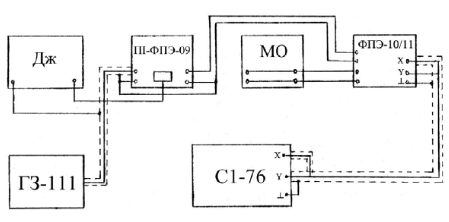
\includegraphics[width=0.5\textwidth]{3.1.png}
        % Підпис (зазвичай під малюнком):
        \caption{Загальна схема досліду}
        % Мітка для посилань у тексті (\ref{fig:...})
        \label{fig1:schema}
    \end{figure}

    %%%%%%%%%%%%%%%%%%%%%%%%%%%%%%%%%%%Теоретичні відомості%%%%%%%%%%%%%%%%%%%%%%%%%%%%%%%%%%%

    \begin{center}
        \textbf{\large Теоретичні відомості}
    \end{center}

    \setlength{\parindent}{1.5em}

    Реальний коливальний контур складається з послідовно з’єднаних конденсатора $C$, котушки індуктивності $L$
    і резистора $R$. Якщо зарядити конденсатор від батареї Б до напруги $U$ (рис. 3.2), а потім від’єднати батарею
    за допомогою ключа $K$, то конденсатор почне розряджатися через котушку і у контурі виникнуть електромагнітні коливання.

    \begin{figure}[h!]

        \renewcommand{\thefigure}{3.\arabic{figure}} % робимо "3.1", "3.2" і т.д.

        \centering
        % Підставляєте потрібний шлях та розмір зображення:
        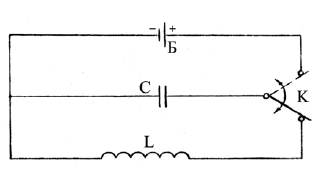
\includegraphics[width=0.5\textwidth]{3.2.png}
        % Підпис (зазвичай під малюнком):
        \caption{Загальна схема досліду}
        % Мітка для посилань у тексті (\ref{fig:...})
        \label{fig2:schema}

    \end{figure}

    Спочатку розглянемо випадок, коли опір контуру $R$ = 0.

    Після замикання контуру в ньому виникне розрядний струм $I$, який не відразу набуває максимального значення.
    Плавна зміна сили струму в колі зумовлена появою в котушці ЕРС самоіндукції, яка за правилом Ленца перешкоджає зміні струму,
    тобто гальмує розряд конденсатора. Як тільки заряд конденсатора стане рівним нулю, сила струму в контурі досягне максимуму.
    З цього моменту сила струму в колі починає зменшуватися, не змінюючи свого напрямку.
    В цьому випадку ЕРС самоіндукції підтримує струм, який викликав її появу.
    Ця ж ЕРС призводить до перезаряджання конденсатора, після чого процес повторюється, однак з іншим напрямом струму.
    Надалі ці процеси повторюються, тобто виникають коливання.

    Час, протягом якого в коливальному контурі відбувається один повний цикл змін і контур повертається в початковий стан, називають періодом електричного коливання.

    Якщо активний опір в контурі дорівнює 0, то коливання в контурі можуть продовжуватися нескінченно довго.
    Такі коливання, які відбуваються внаслідок процесів у самому коливальному контурі без зовнішніх впливів і втрат енергії,
    називають власними електричними коливаннями. Вони є незагасаючими.

    У початковий момент, коли конденсатор був заряджений, у ньому була накопичена енергія

    \begin{center}
        $\displaystyle W_e = \frac{CU^2}{2}.$
    \end{center}

    Під час розрядки енергія електричного поля конденсатора перетворюється в енергію магнітного поля котушки і,
    коли конденсатор повністю розряджений, енергія магнітного поля досягає максимального значення:

    \begin{center}
        $\displaystyle W_m = \frac{LI_0^2}{2}$,
    \end{center}

    де $I_0$ --- амплітуда сили струму в контурі. Під час перезаряджання конденсатора енергія магнітного поля знову перетворюється на енергію електричного поля.
    За умови $R$ = 0 у контурі відбуваються незагасаючі електромагнітні коливання.

    Усі без винятку провідники за звичайних умов мають відмінний від нуля опір, тому частина енергії при
    коливаннях витрачається на їх нагрівання, тобто перетворюється на теплову і втрачається.
    В наслідок цього амплітуда електромагнітних коливань в контурі зменшується
    відбувається загасання коливань (рис. 3.3).

    \begin{figure}[h!]

        \renewcommand{\thefigure}{3.\arabic{figure}} % робимо "3.1", "3.2" і т.д.

        \centering
        % Підставляєте потрібний шлях та розмір зображення:
        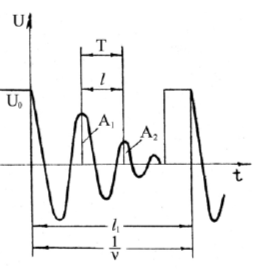
\includegraphics[width=0.3\textwidth]{3.3.png}
        % Підпис (зазвичай під малюнком):
        \caption{Графік згасаючих коливань}
        % Мітка для посилань у тексті (\ref{fig:...})
        \label{fig3:schema}

    \end{figure}

    При достатньо великому опорі контуру або малій індуктивності коливання у ньому взагалі не виникають,
    а відбувається так званий аперіодичний розряд конденсатора.

    Заряд конденсатора і сила струму у котушці коливального контуру постійно змінюються
    за значенням і напрямом. Вважатимемо, що в момент часу $t$ заряд на обкладинках
    конденсатора $q$, напруга на ньому $\displaystyle U_C = \frac{q}{C}$, а сила струму у колі
    змінюється зі швидкістю $\displaystyle \frac{dI}{dt}$. У котушці індуктивності виникає ЕРС самоіндукції

    \begin{equation}
        \mathcal{E}_L = -L\frac{dI}{dt}.
        \tag{3.1}
    \end{equation}

    Відповідно до другого правила Кірхгофа для коливального контуру, опір якого дорівнює нулю, можна записати

    \begin{equation}
        U + \mathcal{E}_L = IR,
        \tag{3.2}
    \end{equation}

    де

    \begin{equation}
        I = -\frac{dq}{dt}.
        \tag{3.3}
    \end{equation}

    (струм тече в додатному напрямку при зменшенні заряду конденсатора).

    Оскільки $q = CU$, то з урахуванням (3.1) та (3.2) отримаємо:

    \begin{center}
        $\displaystyle I = -C \frac{dU}{dt}$,
    \end{center}

    \begin{center}
        $\displaystyle \mathcal{E}_L = LC \frac{d^2U}{dt^2}$.
    \end{center}

    Підставивши останній вираз в (3.2), матимемо:

    \begin{equation}
        \frac{d^2U}{dt^2} + \frac{R}{L} \frac{dU}{dt} + \frac{U}{LC} = 0.
        \tag{3.4}
    \end{equation}

    Як відомо, диференціальне рівняння (3.4) є рівнянням загасаючих електричних коливань.
    Розв’язком цього рівняння є функція

    \begin{equation}
        U = U_0e^{-\beta t} \cos(\omega t + \alpha).
        \tag{3.5}
    \end{equation}

    де $\beta$ --- коефіцієнт загасання,

    \begin{equation}
        \beta = \frac{R}{2L},
        \tag{3.6}
    \end{equation}

    де $\omega$ --- циклічна частота загасаючих коливань,

    \begin{equation}
        \omega = \sqrt{\frac{1}{LC} - \left( \frac{R}{2L}\right)^2}.
        \tag{3.7а}
    \end{equation}

    При цьому

    \begin{equation}
        \omega = \frac{2\pi}{T} \text{  та  } T = \frac{2\pi}{\sqrt{\dfrac{1}{LC} - \left( \dfrac{R}{2L}\right)^2}}.
        \tag{3.7б}
    \end{equation}

    Якщо (3.2) записати у вигляді

    \begin{center}
        $\displaystyle \frac{q}{C} + IR = -\frac{dI}{dt}$
    \end{center}

    та взяти похідну за часом, то отримаємо рівняння подібне до рівняння (3.4):

    \begin{center}
        $\displaystyle \frac{d^2I}{dt^2} + \frac{R}{L} \frac{dI}{dt} + \frac{I}{LC} = 0$.
    \end{center}

    Отже, сила струму $I$ в контурі також здійснює загасаючі коливання (щоправда, початкова фаза цих коливань буде іншою),
    для яких значення $\beta$ й $\omega$ визначаються формулами (3.6), (3.7а) та (3.7б).

    З (3.7а) та (3.7б) видно, що в коливальному контурі можливі загасаючі коливання лише у випадку,
    якщо $\displaystyle \frac{1}{LC} > \left( \frac{R}{2L}\right)^2$ (частота та період є дійсними величинами)
    або $\displaystyle R < 2\sqrt{\frac{L}{C}}$, то частота і період – уявні величини, коливань немає і відбувається
    аперіодичний розряд конденсатора.

    Опір

    \begin{equation}
        R_K = 2\sqrt{\frac{L}{C}}
        \tag{3.8}
    \end{equation}

    називають критичним.

    Щоб характеризувати загасаючі коливання, окрім коефіцієнта загасання $\beta$,
    використовується ще логарифмічний декремент (лат. dekrement --- зменшення) загасання.

    Логарифмічним декрементом загасання називається натуральний логарифм
    відношення значень напруги, розділених інтервалом часу,
    який дорівнює періоду коливань $T$,

    \begin{equation}
        \lambda = \ln \frac{A_1}{A_2} = \ln \frac{A(t)}{A(t+T)},
        \tag{3.9}
    \end{equation}

    або

    \begin{center}
        $\displaystyle \lambda \approx 2,3\cdot \lg \frac{A_1}{A_2}$.
    \end{center}

    Підставивши в (3.9) значення $A(t) = U_0e^{-\beta t}$ та $A(t+T) = U_0e^{-\beta (t+T)}$, отримаємо

    \begin{equation}
        \lambda = \beta T,
        \tag{3.10}
    \end{equation}

    або згідно (3.6)

    \begin{equation}
        \lambda = \frac{R}{2L}T.
        \tag{3.10а}
    \end{equation}

    У деяких випадках зручно вивчати коливний процес у системі координат $I$ та $U$,
    тобто відкладати на осі абсцис значення сили струму в контурі,
    а на осі ординат -- напругу на конденсаторі у той же момент часу.
    Площина $IU$ має назву площини станів, або фазової площини, а крива,
    яка зображає залежність напруги від струму, називається фазовою кривою (див. рис. 3.4).

    \begin{figure}[h!]

        \renewcommand{\thefigure}{3.\arabic{figure}} % робимо "3.1", "3.2" і т.д.

        \centering
        % Підставляєте потрібний шлях та розмір зображення:
        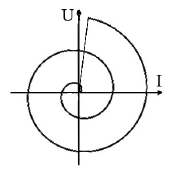
\includegraphics[width=0.3\textwidth]{3.4.png}
        % Підпис (зазвичай під малюнком):
        \caption{Фазова крива}
        % Мітка для посилань у тексті (\ref{fig:...})
        \label{fig4:schema}

    \end{figure}

    Знайдемо фазову криву для контуру, опір якого $R = 0$. цьому випадку
    $\beta = \frac{R}{2L} = 0$ і тоді з (3.5), (3.7а) та (3.7б) отримуємо

    \begin{equation}
        \omega = \sqrt{\frac{1}{LC}},\text{ } T = 2\pi \sqrt{LC},
        \tag{3.11}
    \end{equation}

    \begin{equation}
        \left\{
        \begin{aligned}
            U &= U_0 \cos \omega t \\
            I &= -C \frac{dU}{dt} = U_0 \omega C \sin \omega t
        \end{aligned}
        \right.
        \tag{3.12}
    \end{equation}

    Рівняння (3.11), (3.12) описують незагасаючі коливання.
    Виключивши з них час $t$, отримаємо рівняння фазової кривої (рівняння еліпса):

    \begin{center}
        $\displaystyle \frac{U^2}{U_0^2} - \frac{I^2}{U_0^2 \omega^2 C^2} = 1$.
    \end{center}

    Еліпс можна отримати у результаті накладання двох взаємно перпендикулярних
    гармонічних коливань (3.12), із зсувом фаз у чверть періоду.

    У контурі, опір якого $R>0$, відбуваються загасаючі коливання напруги (3.5) та струму:
    \begin{center}
        $
        \left\{
        \begin{aligned}
            U &= U_0 e^{-\beta t} \cos \omega t \\
            I &= -C \frac{dU}{dt} = U_0C e^{-\beta t} (\beta \cos \omega t + \omega \sin \omega t)
        \end{aligned}
        \right.
        $
    \end{center}

    У цьому випадку амплітуди напруги та сили струму у контурі безперервно
    спадають і фазова крива буде незамкненою (рис.3.4).

    У даній роботі для отримання коливань у контурі використовується касета
    ФПЕ-10/11 з контуром, зображеним на рис. 3.5.

    \begin{figure}[h!]

        \renewcommand{\thefigure}{3.\arabic{figure}} % робимо "3.1", "3.2" і т.д.

        \centering
        % Підставляєте потрібний шлях та розмір зображення:
        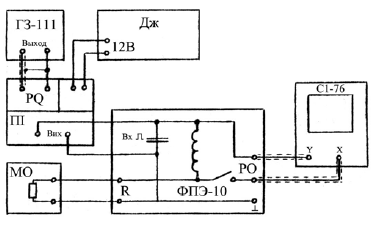
\includegraphics[width=0.5\textwidth]{3.5.png}
        % Підпис (зазвичай під малюнком):
        \caption{Схема експериментальної установки}
        % Мітка для посилань у тексті (\ref{fig:...})
        \label{fig5:schema}

    \end{figure}

    Загасаючі коливання, які відбуваються у контурі, спостерігаються на екрані
    осцилографа С1-76. Цикл зарядки та розрядки конденсатора продовжується
    протягом часу $T = \dfrac{1}{v}$, де $v$ – частота, яка задається звуковим
    генератором ГЗ-111. На екрані осцилографа йому відповідає відрізок $l_1$.
    Це дозволяє визначити період $T$ загасаючих коливань,
    якому на рис. 3.3 відповідає відрізок l. З пропорції $\dfrac{l}{T} = l_1v$ отримаємо

    \begin{equation}
        T = \frac{l}{l_1v}.
        \tag{3.14}
    \end{equation}

    %%%%%%%%%%%%%%%%%%%%%%%%%%%%%%%%%%%Теоретичні відомості%%%%%%%%%%%%%%%%%%%%%%%%%%%%%%%%%%%

    \newpage

    \begin{center}
        \textbf{\large Практична частина}
    \end{center}

    %\begin{equation}
        %W_e = \frac{C U^2}{2}
        %\tag{}
    %\end{equation}

\end{document}